%%% Local Variables: 
%%% mode: latex
%%% TeX-master: t
%%% End: 

\chapter{实验对比与分析}
\label{cha5}

\section{骨架对齐误差度量}
对一幅参考图像和一幅待配准图像来说,各自最多存在14个骨架化分割结果,最多有7种环结构组合(三点环、四点环、五点环、三四点环、三五点环、四五点环、三四五点环),因此在我们提出的配准方法中,最多共有$14\times14\times7$个局部-全局配准结果,如流程图所示。

然后,我们需要对配准结果进行准确性评估,除了采用人工对配准结果进行估计,还需要考虑采用客观的定量估计方法。然而,现今视网膜图像配准领域并没有统一的配准结果评价方法,常见的配准准确性评估方法有匹配误差和对齐误差等,其中CEM(中心线误差估计)~\cite{can}是常用的一种视网膜配准结果估计算法。

所谓中心线误差度量(CEM)误差,指的是参考图像与变换后的待配准图像血管中心线的平均距离。这种方法需要对图像进行分割、通过轨迹回归追踪算法以得到血管中心线。对于参考图像的每一个血管中心点($P_m$),寻找变换后的待配准图像中与之距离最近的中心线点($P_n$,该点与$P_m$组成一对对应点),计算距离,然后求得两幅图像的所有血管中心线点距离的中值作为标准。公式如下:
\begin{align}
CEM_i  = Median(P_{mj}-P_{nj})\quad j=1,2,\ldots,n
\end{align}
最后,如果对多幅视网膜图像误差进行计算,可以求得这些图像的CEM值的平均值,即平均中心线误差:
\begin{align}
E=average(CEM_i)\quad i=1,2,\ldots,m
\end{align}
		
考虑到视网膜图像的特性,及我们算法过程的特点,我们提出了成功率(Success Rate)和骨架化对齐误差估计(Skeleton Alignment Error Measure)算法来度量配准结果的准确性,同时通过极小化SAEM来自动选择最优配准结果。

所谓成功率(SR)指的是配准成功的结果占所有配准的结果的比率。其中关于配准结果的判断,一是配准的SAEM需小于一定阈值(1.5个像素),二是通过人工判别判断满足配准成功的标准。

从我们观察来看,一个好的配准结果是拥有较高血管重合率的配准结果。然而,因为参考图像与待配准图像的处理方法不同,待配准图像变换后的血管网络会出现检测到的血管是不连续的情况,即有些血管上的点不存在,这是因为变换后所有点的坐标我们取的都是整数值,因此有些点变换后可能没有对应点。为了尽量减少上述情况的影响,我们在求SAEM时,以待配准图像变换后的图像作为求取血管点距离的参考图像。SAEM的思路是通过在参考血管点周围设定一个固定大小的window,来计算该window内与其距离最小的点并将其作为对应点,最后求得所有对应血管点的距离平均值作为结果。算法流程如下:
\begin{enumerate}
\item 对于给定的一幅参考图像的骨架化结果$M_i(i=1,2,\ldots,14)$,和其对应的待配准图像骨架化结果$N_j(j=1,2,\ldots,14)$,每幅$N_j$用一种多环结构$L_k(k=1,2,\ldots,7)$在局部-全局配准策略下进行配准,得到的变换后的骨架化图像为$N_{jM_i}$。
\item 对于$N_{jM_i}$中的每个血管点,以其为中心取$7\times7$的一个区域(window),计算在$M_i$对应区域内与该血管点距离最近的$M_i$上的点。我们将该点认为是$N_{jM_i}$中的血管点的对应点,两者之间的距离为欧氏距离$d$。若在区域内不存在对应的血管点,则将$N_{jM_i}$中的该血管点标记为无效点。
\item 计算完成$N_j$的所有点,得SAEM定义如下:
\begin{align}
SAEM_{ijk}=\frac{(\sum d)}{Num_v}
\end{align}	 	
其中$Num_v$是$N_{jM_i}$的有效像素数。
\item 约束条件为$\frac{Num_v}{Num_{N_j}}$,并且$\frac{Num_{N_jM_i}}{Num_{N_j}}\geq 38\%$ ,其中$Num_{(.)}$代表$(.)$中的像素数量。
\end{enumerate}

约束条件是为了防止某些极端情况:配准结果的血管点有效率较低,大部分血管出现严重偏离;或配准结果出现形变,只有极少数的能够配准的点,但这些点的有效率较高。因此我们从血管点有效率和配准变换后的图像像素数占原始图像像素数的比例两个方面进行约束,以杜绝极端的、不合格的配准结果,其中阈值的设定由实验与人工观察的结果得出。

通过使用SAEM,视网膜图像的配准结果可以进行定量的分析,而且最优配准结果可以智能的选择出来,同时我们还可以得到参考图像与待配准图像的对应的分割序号,及最优的环结构组合。算法的所有过程如流程图中所示,我们提出的基于多尺度和多环特征的从局部到全局的配准策略,通过骨架化对齐误差的估计,不仅排除了人工选择分割结果可能造成的配准特征提取失败从而影响后续配准结果的现象,实现了分割尺度和环结构的自动选择,而且最大限度的保证了配准结果的准确性,真正实现了配准结果的最优化。后续的对比试验及结果分析会进一步说明我们提出的配准算法的优越性。
\section{数据集}
我们需要一个完整的视网膜数据集进行实验以验证我们配准算法的有效性,但目前网上存在很少的用于配准目的的视网膜图像数据集。因此我们选用VARIA数据库~\cite{ortega}\cite{ortega1},一个用来做图像鉴别的视网膜图像库,作为从定性和定量两个方面评价和估计我们视网膜配准算法的数据集。VARIA数据集,目前包含了233幅视网膜图像,来自于139个采集者。这些图像均由日本拓普康眼底NW-100模型照相机获取,为了保证视网膜图像采集时,瞳孔不会随光线发生变化,采用散瞳化处理。同时获取时尽量以视神经盘为中心进行处理,最终的图像分辨率为$768\times584$。

在139个采集者中,每个个体有不同数量的采集图像,因此同一个个体可能有多对用于配准的图像,经过我们两两配对,最终得到了155对视网膜图像用于进行配准。

图~\ref{twiceresult}中为一组视网膜图像的配准结果示例图。其中(a)和(b)是原始视网膜图像,(c)和(d)分别为局部初始配准结果和全局最终配准结果,(e)为最终的原始图像配准结果。我们可以看到未对齐的血管经过局部到全局的配准策略已经得到了较精确地匹配。

\begin{figure}
\centering
\begin{minipage}[b]{0.45\linewidth} 
      \centering 
      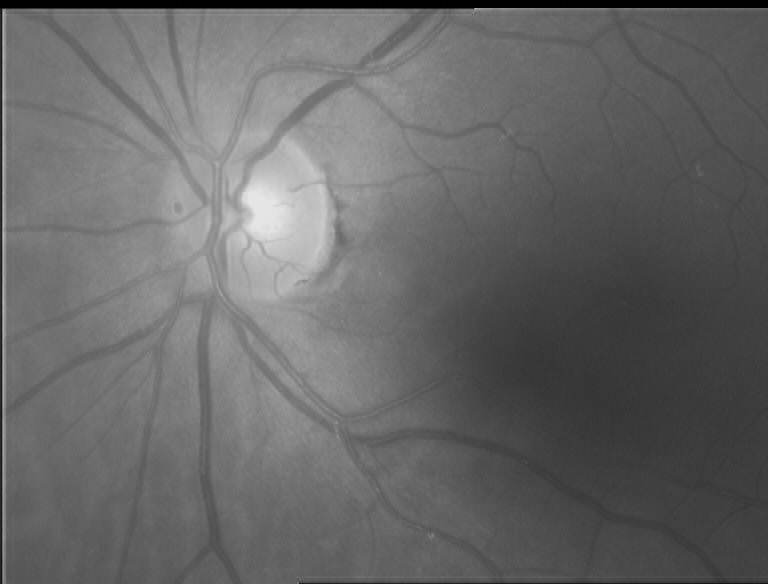
\includegraphics[width=0.9\linewidth]{R160.png}
        \centerline{(a) 参考图像}\medskip
\end{minipage}
  \begin{minipage}[b]{0.45\linewidth}
    \centering
    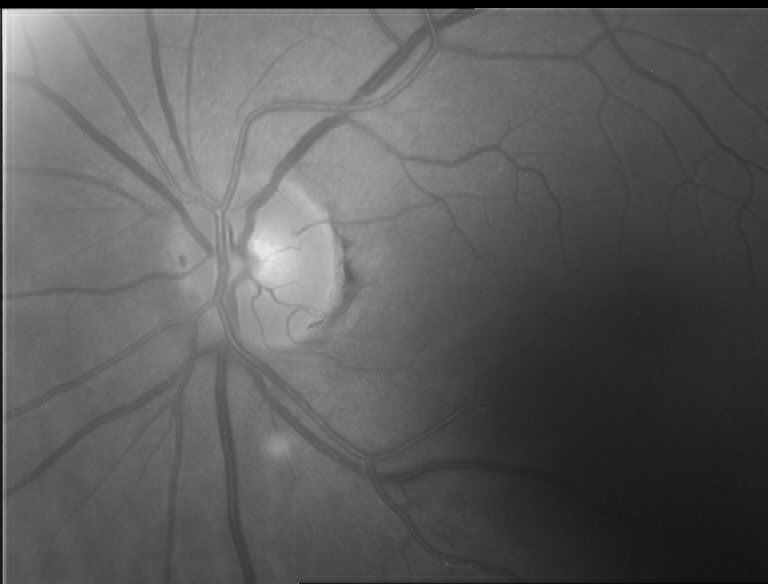
\includegraphics[width=0.9\linewidth]{R161.png}
      \centerline{(b) 待配准图像}\medskip
  \end{minipage}
    \begin{minipage}[b]{0.45\linewidth}
    \centering
    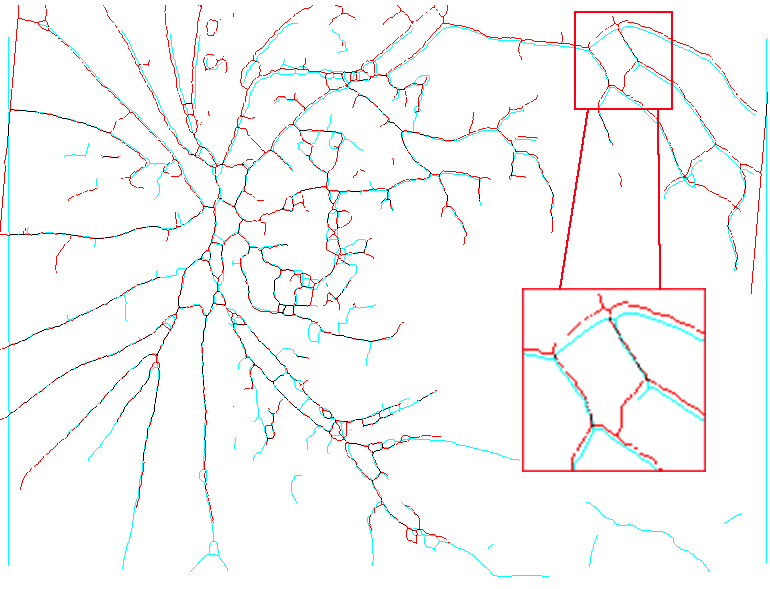
\includegraphics[width=0.9\linewidth]{160-161-initial.png}
      \centerline{(c) 局部初始骨架化配准结果}\medskip
  \end{minipage}
  \begin{minipage}[b]{0.45\linewidth}
    \centering
    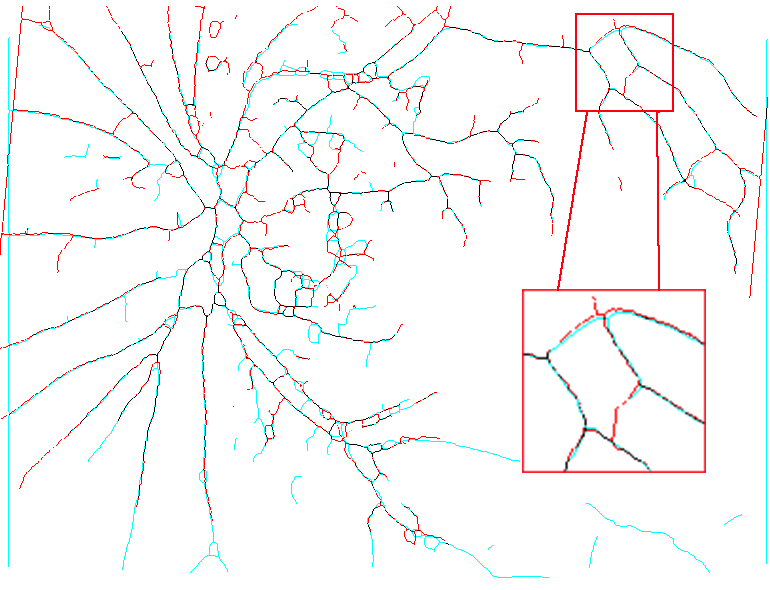
\includegraphics[width=0.9\linewidth]{160-161-local.png}
      \centerline{(d) 全局二次骨架化配准结果}\medskip
  \end{minipage}
   \begin{minipage}[b]{0.45\linewidth}
    \centering
    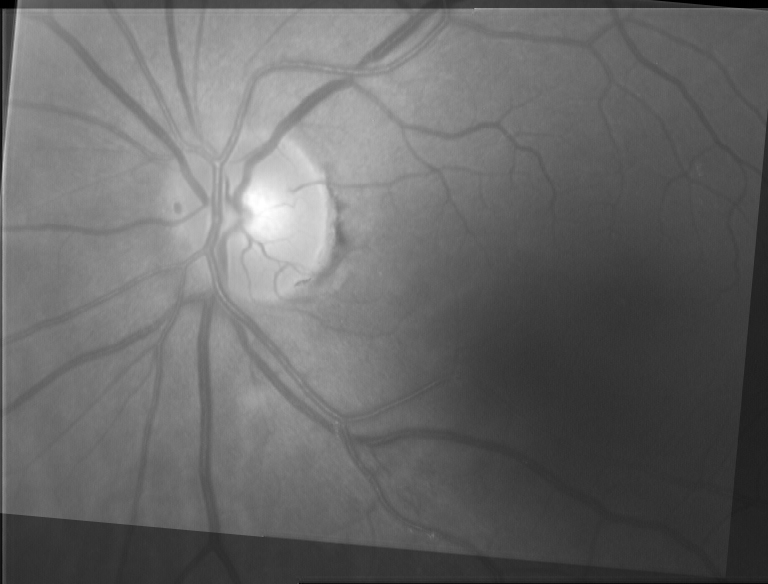
\includegraphics[width=0.9\linewidth]{160-161-result.png}
      \centerline{(e) 全局二次原始图像配准结果}\medskip
  \end{minipage}
 \caption{局部与全局配准结果}
\label{twiceresult}
\end{figure}


\section{对比实验}
我们提到由成功率(SR)和骨架化对齐误差(SAEM)来对配准结果进行估计,其中成功与否需满足两个条件,判定配准失败的结果并不计入到SAEM中。
\subsection{变换模型对比}
变换模型的选择对于配准来说是十分重要的,上一章中讨论了对于不同配准特征变换模型的重要性,这里实验结果表明了不同的变换模型对于我们的环结构的配准结果影响。实验中选择了只用环结构得到的配准结果中对应的最优尺度和最优环结构作为配准特征,选择了相似性变换,仿射变换和二阶多项式变换作为变换模型,由MATLAB的\emph{cp2tform}函数实现。
\begin{table}[!h]
\caption{不同变换模型的对比结果}
\centering
\begin{tabular}{lcc}
\toprule
变换模型 & 成功率(SR)& SAEM (单位:像素)\\
\midrule
相似性变换 & $\mathbf{95.5\%}$ & $\mathbf{0.9206}$ \\
仿射变换 & $35.48\%$ & $0.844$              \\
多项式变换& $15.48\%$ & $0.139$\\
\bottomrule
\end{tabular}
\label{models}
\end{table}
从表格~\ref{models}结果可以观察到,虽然多项式变换的SAEM低至0.139个像素,但其配准成功率只有$15.48\%$,这是因为配准失败的例子并不计算在SAEM内,同时说明多项式变换对环结构来说是不合适的,究其原因,多项式变换极易在远离控制点的区域造成图像扭曲的现象,如图~\ref{3model}所示的三种变换模型的对比中多项式所对应的结果。上述数据显示,相似性变换拥有最高的成功率$95.5\%$和0.9206像素的SAEM,其更符合环结构的构造原理,因此被我们选作变换模型。
\begin{figure}
\centering
\begin{minipage}[b]{0.45\linewidth} 
      \centering 
      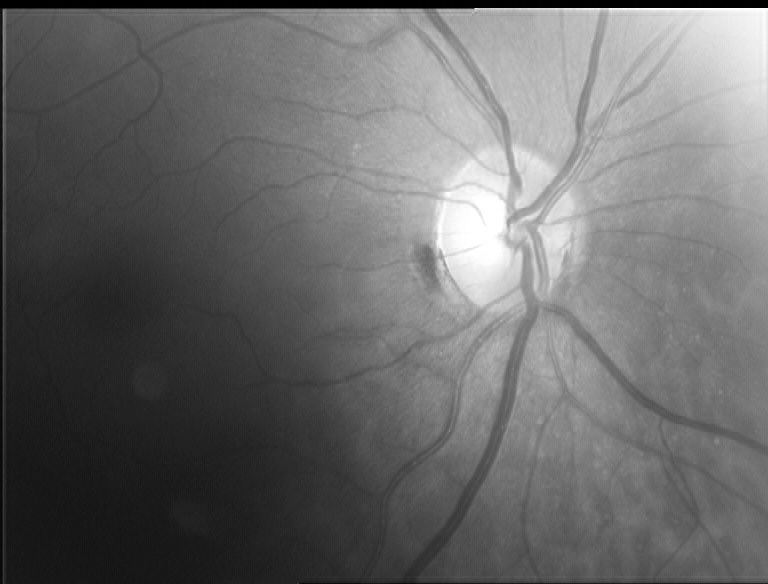
\includegraphics[width=0.9\linewidth]{R132.png}
        \centerline{(a) 参考图像}\medskip
\end{minipage}
  \begin{minipage}[b]{0.45\linewidth}
    \centering
    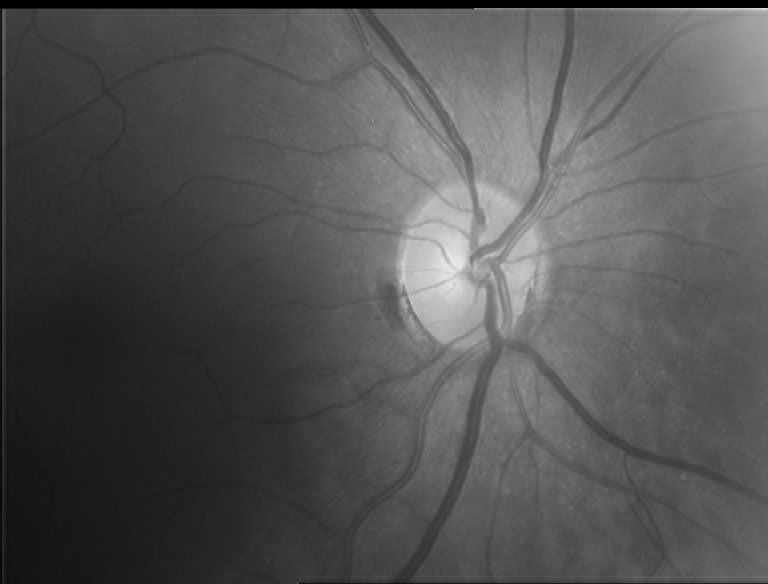
\includegraphics[width=0.9\linewidth]{R133.png}
      \centerline{(b) 待配准图像}\medskip
  \end{minipage}
    \begin{minipage}[b]{0.45\linewidth}
    \centering
    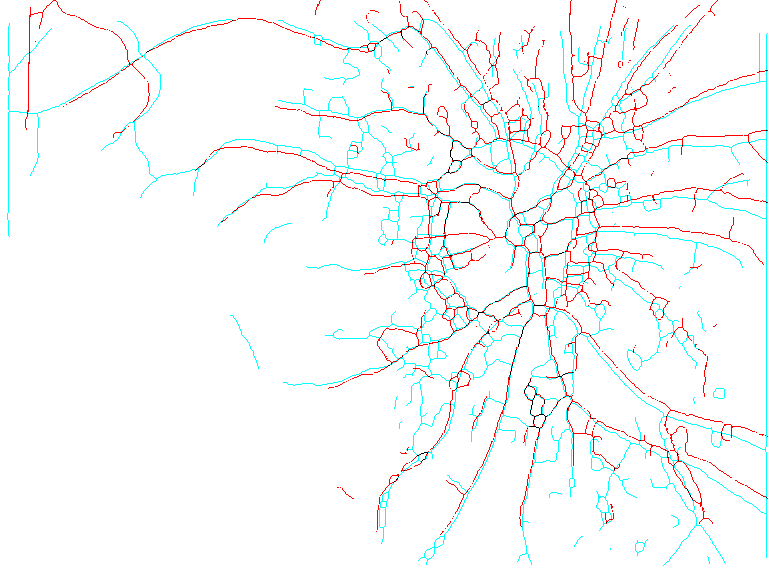
\includegraphics[width=0.9\linewidth]{R132-R133-4-3-affine-three_five-1.7024.png}
      \centerline{(c) 仿射变换骨架化配准结果}\medskip
  \end{minipage}
  \begin{minipage}[b]{0.45\linewidth}
    \centering
    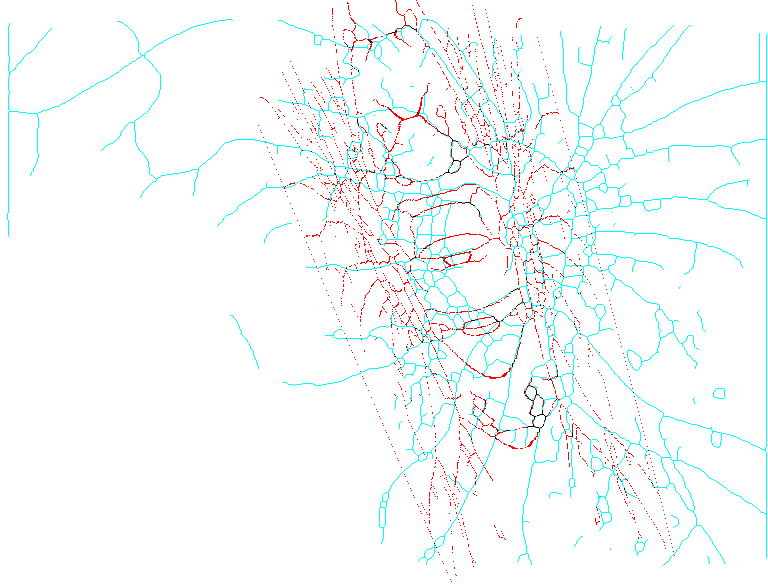
\includegraphics[width=0.9\linewidth]{R132-R133-4-3-polynomial-three_five-13.png}
      \centerline{(d) 多项式变换骨架化配准结果}\medskip
  \end{minipage}
   \begin{minipage}[b]{0.45\linewidth}
    \centering
    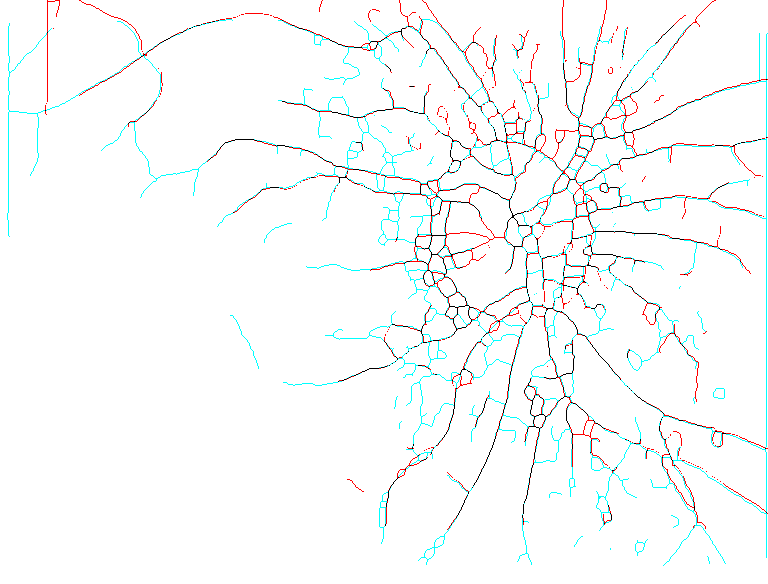
\includegraphics[width=0.9\linewidth]{R132-R133-4-3-similarity-three_five-0.84855.png}
      \centerline{(e) 相似性变换骨架化配准结果}\medskip
  \end{minipage}
 \caption{不同变换模型配准结果}
\label{3model}
\end{figure}


\subsection{特征对比}
然后我们对局部到全局的配准过程中的不同特征进行了对比,三个特征分别为环,环-血管,环-血管-分叉点。三种方法均使用了多尺度的分割方法,采用相似性变换作为变换模型,对共计155组视网膜图像进行了处理,结果如下:
\begin{table}[!ht]
\caption{不同特征的对比试验结果}
\centering
\begin{tabular}{lcc}
\toprule
特征 & 成功率(SR)& SAEM (单位:像素)\\
\midrule
环特征 & $95.5\%$ & $0.921$ \\
环-血管特征 & $96.77\%$ & $0.895$              \\
环-血管-分叉点特征& $\mathbf{100\%}$ & $\mathbf{0.873}$\\
\bottomrule
\end{tabular}
\label{features}
\end{table}

由表~\ref{features}中数据可知,从环特征,环-血管特征,再到环-血管-分叉点特征,配准结果的成功率和SAEM值都有了局部的提高,环-血管-分叉点特征是其中最具鲁棒性的特征。
一些关于环,环-血管,环-血管-分叉点的图像对比结果如图~\ref{feature-comp1}和~\ref{feature-comp2}所示。
\begin{figure}
\centering
\begin{minipage}[b]{0.45\linewidth} 
      \centering 
      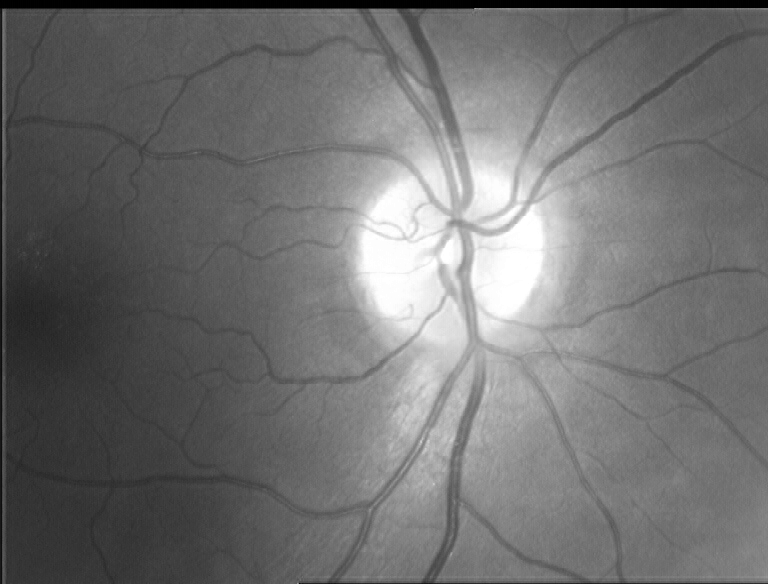
\includegraphics[width=0.9\linewidth]{R118.png}
        \centerline{(a) 参考图像}\medskip
\end{minipage}
  \begin{minipage}[b]{0.45\linewidth}
    \centering
    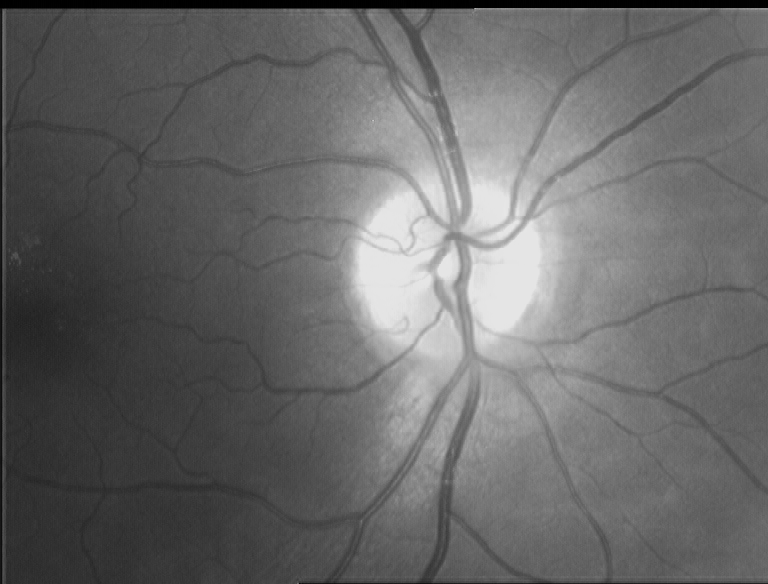
\includegraphics[width=0.9\linewidth]{R119.png}
      \centerline{(b) 待配准图像}\medskip
  \end{minipage}
    \begin{minipage}[b]{0.45\linewidth}
    \centering
    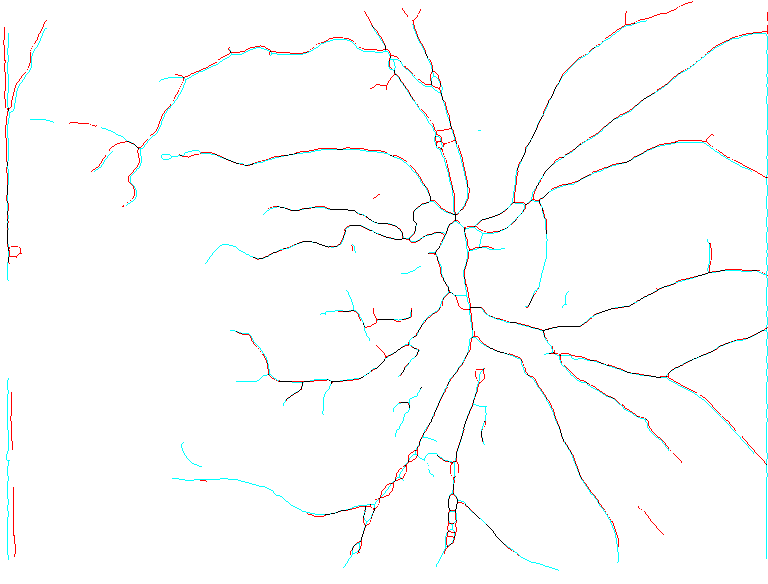
\includegraphics[width=0.9\linewidth]{R118-R119-8-9-cycle-four_five-0.90055.png}
      \centerline{(c) 环特征骨架化配准结果}\medskip
  \end{minipage}
  \begin{minipage}[b]{0.45\linewidth}
    \centering
    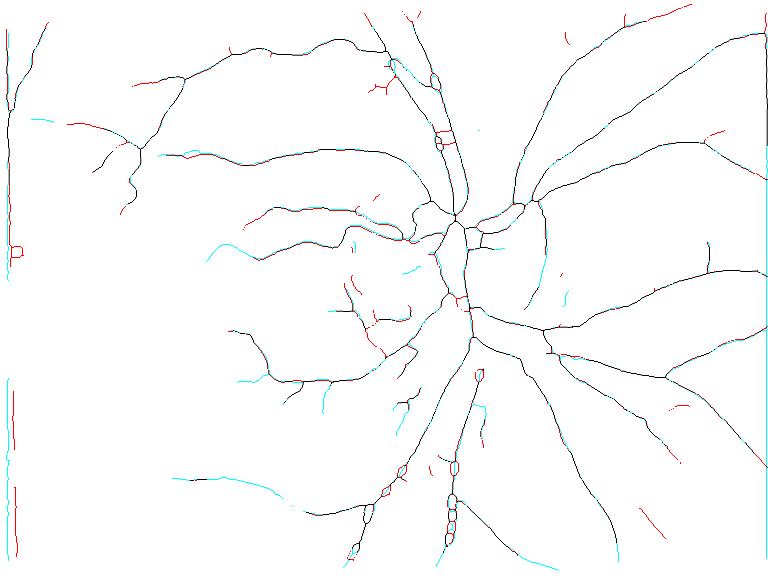
\includegraphics[width=0.9\linewidth]{R118-R119-10-6-vessel-three_four-0.64047.png}
      \centerline{(d) 环-血管特征骨架化配准结果}\medskip
  \end{minipage}
   \begin{minipage}[b]{0.45\linewidth}
    \centering
    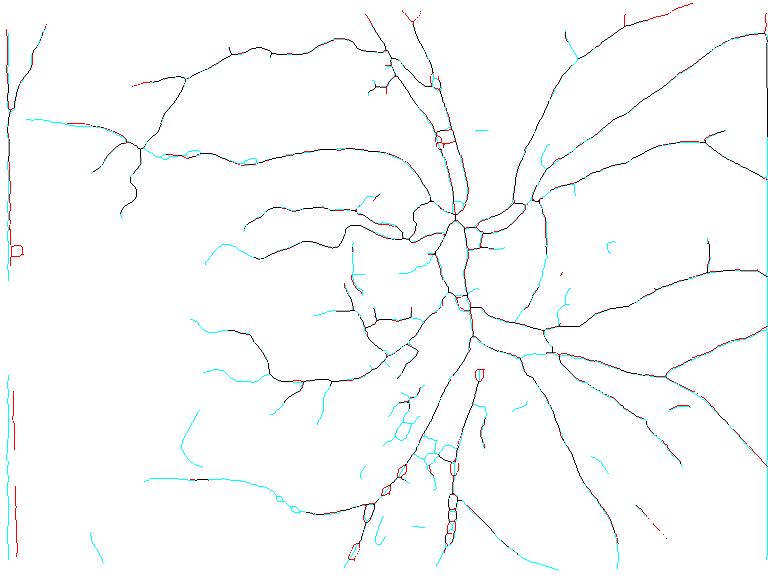
\includegraphics[width=0.9\linewidth]{R118-R119-2-6-twice-14-three_four-0.5855.png}
      \centerline{(e) 环-血管-分叉点特征骨架化配准结果}\medskip
  \end{minipage}
 \caption{不同特征配准结果一}
\label{feature-comp1}
\end{figure}

\begin{figure}
\centering
\begin{minipage}[b]{0.45\linewidth} 
      \centering 
      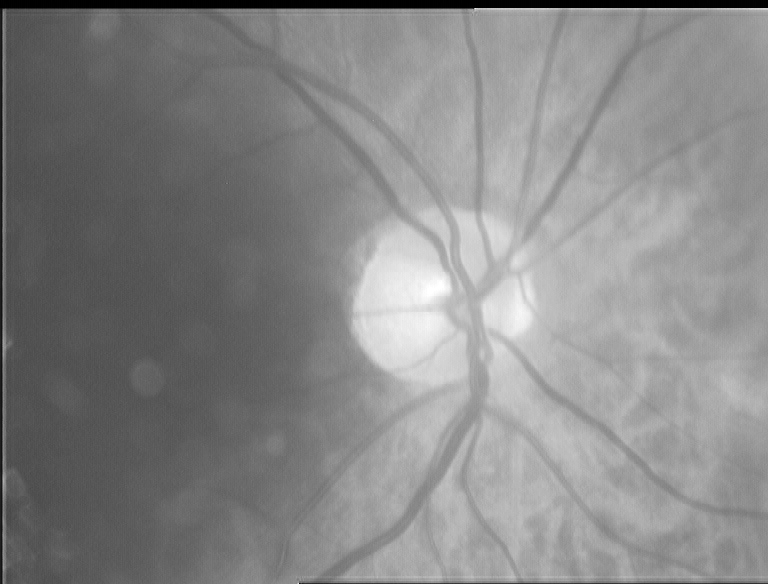
\includegraphics[width=0.9\linewidth]{R120.png}
        \centerline{(a) 参考图像}\medskip
\end{minipage}
  \begin{minipage}[b]{0.45\linewidth}
    \centering
    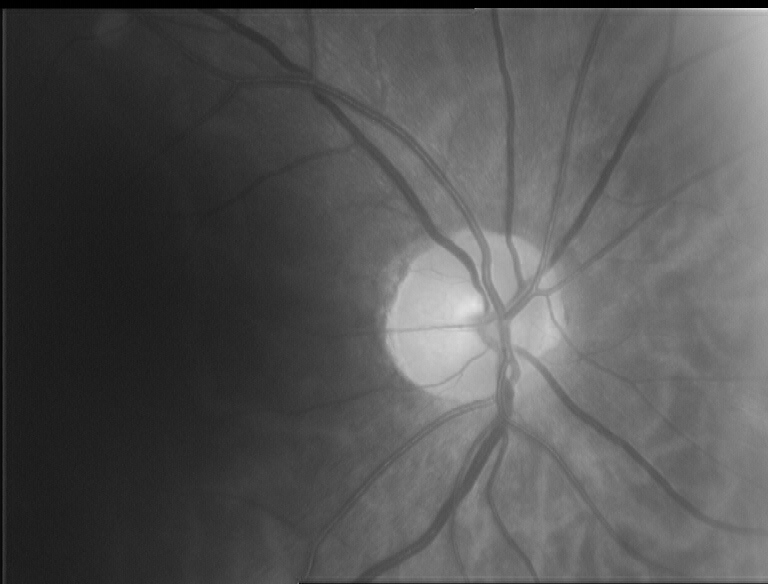
\includegraphics[width=0.9\linewidth]{R121.png}
      \centerline{(b) 待配准图像}\medskip
  \end{minipage}
    \begin{minipage}[b]{0.45\linewidth}
    \centering
    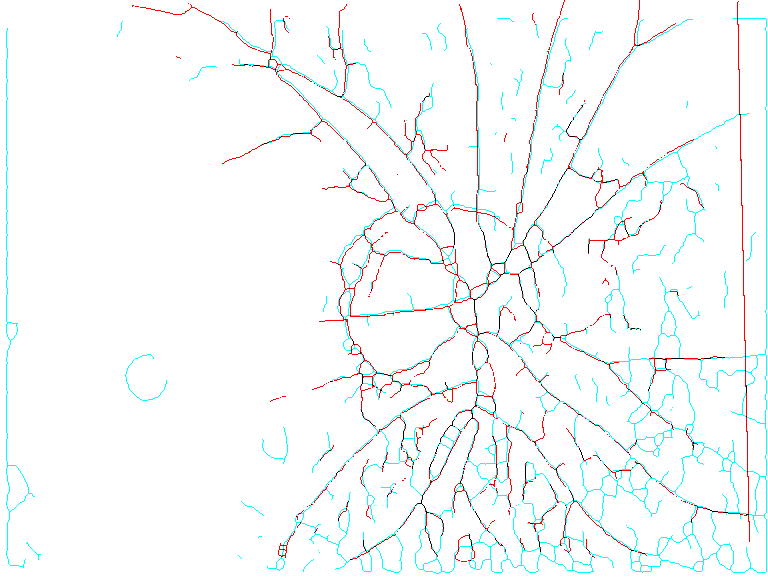
\includegraphics[width=0.9\linewidth]{R120-R121-12-6-cycle-four_five-1.2545.png}
      \centerline{(c) 环特征骨架化配准结果}\medskip
  \end{minipage}
  \begin{minipage}[b]{0.45\linewidth}
    \centering
    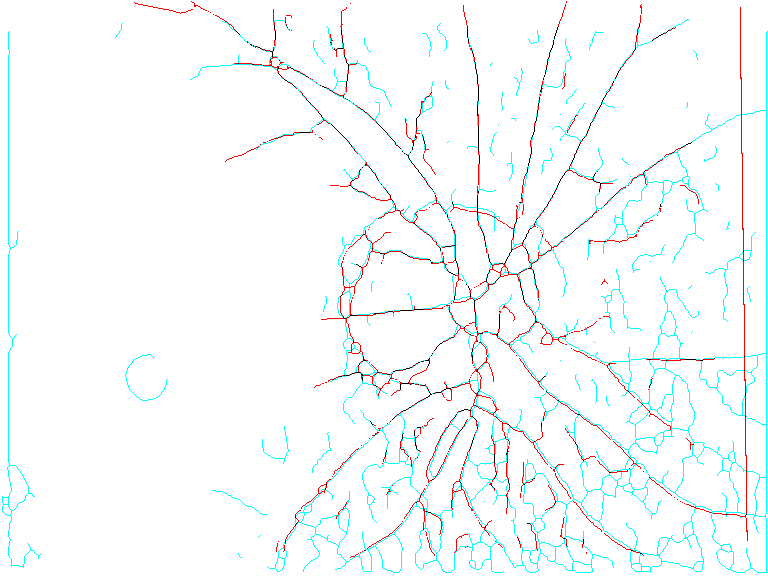
\includegraphics[width=0.9\linewidth]{R120-R121-7-1-vessel-four-1.1862.png}
      \centerline{(d) 环-血管特征骨架化配准结果}\medskip
  \end{minipage}
   \begin{minipage}[b]{0.45\linewidth}
    \centering
    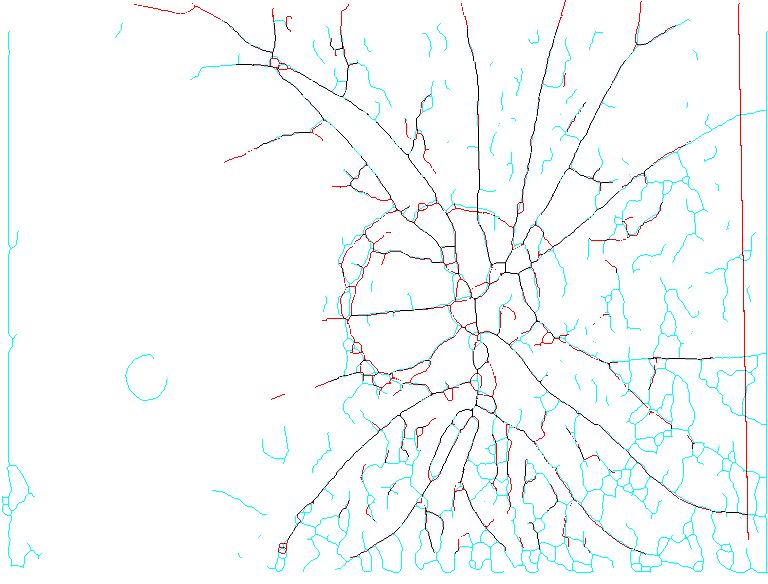
\includegraphics[width=0.9\linewidth]{R120-R121-7-5-twice-14-four-0.94365.png}
      \centerline{(e) 环-血管-分叉点特征骨架化配准结果}\medskip
  \end{minipage}
 \caption{不同特征配准结果二}
\label{feature-comp2}
\end{figure}


\subsection{算法对比}
我们首先进行了二级配准结果与三步特征选择的对比试验,结果如下。
\begin{table}[!ht]
\caption{二级配准与三步特征选择的对比实验结果}
\centering
\begin{tabular}{lcc}
\toprule
方法& 成功率(SR)& SAEM (单位:像素)\\
\midrule
二级配准 & $100\%$ & $0.873$ \\
三步特征选择 & $100\%$ & $0.858$ \\        
\bottomrule
\end{tabular}
\label{methods1}
\end{table}

由表格~\ref{methods1}可知,三步特征选择的实验结果优于二级配准结果,这也符合我们的预期,说明在某些情况下,仅使用简单的环结构,或者经过初次局部配准,就可以取得最优的配准结果,更多特征点的加入反而会给配准结果造成负面的影响,可能的原因是后加入的特征点精度存在问题,或者是在变换模型下,不同区域的特征点对参数的得出具有一定的影响。另外我们对三步特征选择中各特征的比率进行统计:在155组配准图像中,最优结果为环特征的占$25.8\%$,为环-血管特征的占$10.97\%$,为环-血管-分叉点的占$63.2\%$。由此可得,环-血管-分叉点特征下的二级配准仍然是最具稳定性的方法。

然后,我们将我们提出的视网膜配准方法与现今效果最好的结构匹配方法:Bifurcation结构方法进行对比~\cite{chen}。因为Bifurcation结构中并没有关于图像分割的具体方法,而我们也无法找到一个统一的公正的分割结果作为以上配准方法的输入,所以我们采用我们提出的多尺度的概念,对155组视网膜图像,应用以上三种方法进行陪准实验。同时我们为了验证提出的全局二次配准的作用,将Bifurcation结构与我们的二次配准方法相结合,进行了对比实验。实验结果展示在表格~\ref{methods2}中。
\begin{table}[!ht]
\caption{不同方法的对比实验结果}
\centering
\begin{tabular}{lcc}
\toprule
方法 & 成功率(SR)& SAEM (单位:像素)\\
\midrule
Bifurcation 结构& $95.5\%$ & $0.937$ \\
Bifurcation 结构+Global & $96.77\%$ & $0.877$ \\
我们的方法& $\mathbf{100\%}$ & $\mathbf{0.873}$\\
\bottomrule
\end{tabular}
\label{methods2}
\end{table}

从上述数据可知,我们提出的方法在两个方面的表现超过了bifurcation结构的方法:第一,同样是应用最优的分割结果,也就是不考虑分割方法,同时在应用全局二次变换的情况下(见表格~\ref{methods2}的三、四行),我们的方法比Bifurcation的方法在成功率及SAEM度量方面都要好,由此说明我们提出的环结构特征比Bifurcation结构更加稳定,更具有唯一性与鲁棒性;第二,我们提出了多尺度与从局部到全局的配准策略,大大提高了Bifurcation结构的配准准确性。作为结构特征,Bifurcation结构对分割结果的准确性要求比较高,较差的分割结果无法提取出足够数量和准确的Bifurcation结构,尤其在视网膜图像血管比较稀疏的情况下。实验表明,在较随机抽取的分割结果下,Bifurcation结构并不能取得很好的结果,而通过我们的多尺度分割方法,大大减轻了因分割结果不理想造成的特征提取不符合期望的情况,最终配准结果准确率的提高也证明了这一点。而通过Bifurcation与全局二次配准方法的结合,最终配准的成功率和SAEM又有了显著的提高,证明了我们提出的全局二次配准策略具有较好的效果和通用性。对于一些其他结构特征的改进和提高,具有较高的参考价值。

一些关于三种方法的对比实验结果如图~\ref{m1}和~\ref{m2}所示.
\begin{figure}
\centering
\begin{minipage}[b]{0.42\linewidth} 
      \centering 
      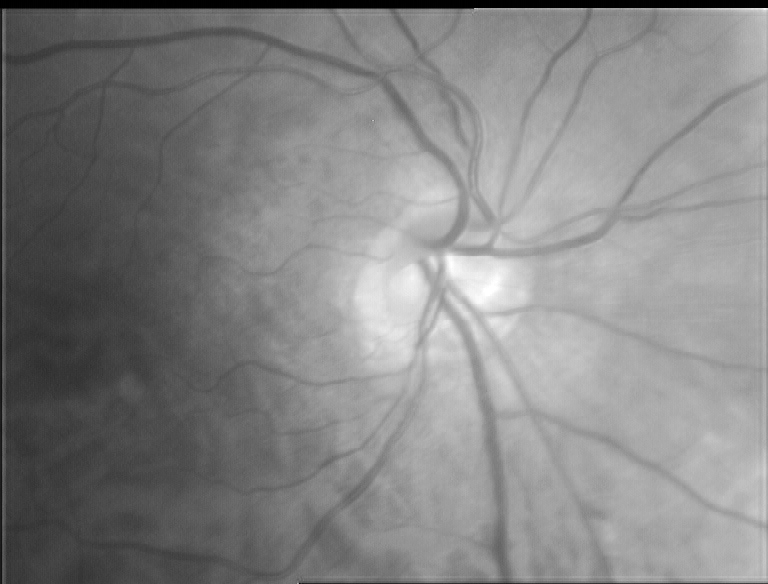
\includegraphics[width=0.9\linewidth]{R122.png}
        \centerline{\footnotesize{(a) 参考图像}}\medskip
\end{minipage}
  \begin{minipage}[b]{0.42\linewidth}
    \centering
    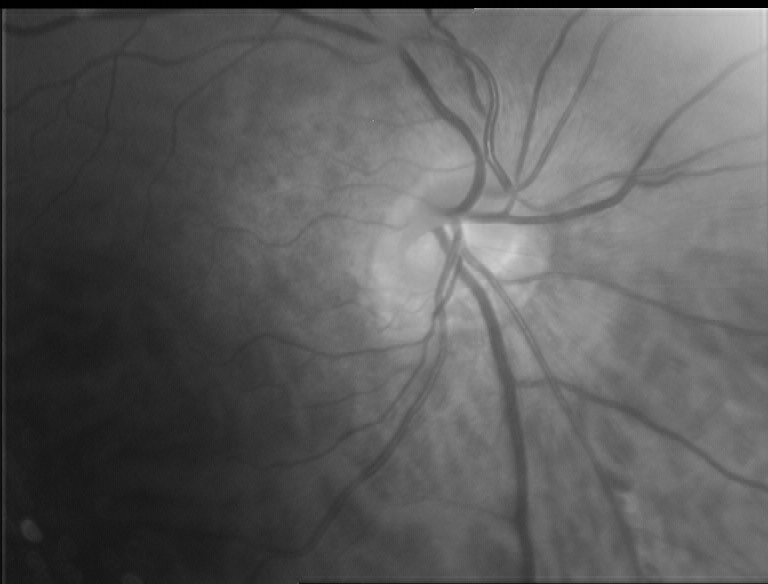
\includegraphics[width=0.9\linewidth]{R123.png}
      \centerline{\footnotesize{(b) 待配准图像}}\medskip
  \end{minipage}
  \\
    \begin{minipage}[b]{0.42\linewidth}
    \centering
    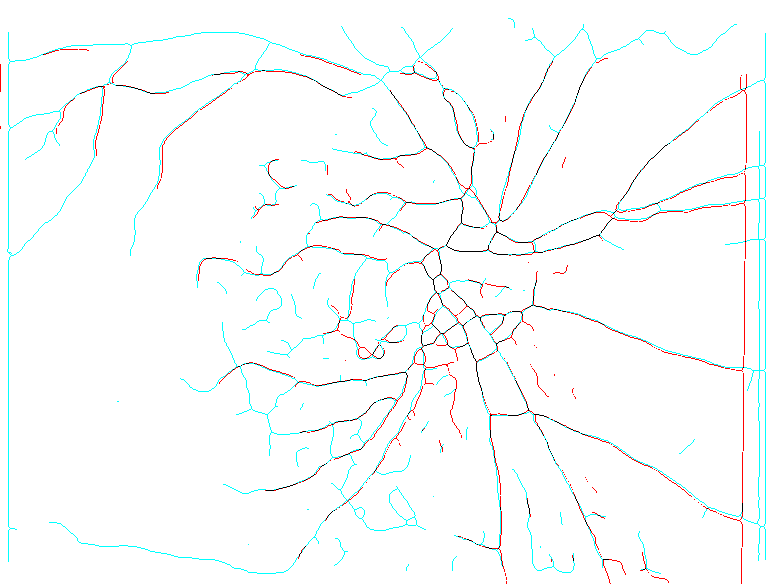
\includegraphics[width=0.9\linewidth]{R122R123-Bifurcation-Skeleton-Registration-1.0068.png}
      \centerline{\footnotesize{(c) Bifurcation方法骨架化配准结果}}\medskip
  \end{minipage}
      \begin{minipage}[b]{0.42\linewidth}
    \centering
    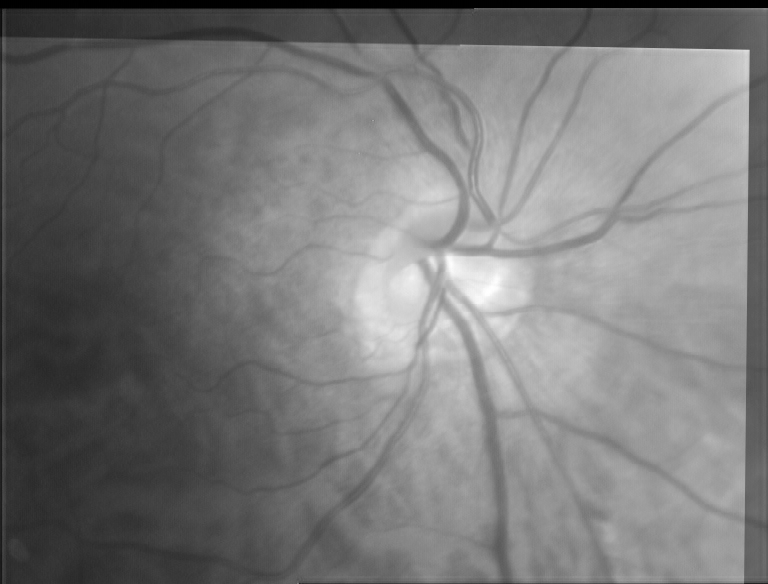
\includegraphics[width=0.9\linewidth]{R122R123-Bifurcation-Registration.png}
      \centerline{\footnotesize{(d) Bifurcation方法原始图像配准结果}}\medskip
  \end{minipage}
    \\
  \begin{minipage}[b]{0.42\linewidth}
    \centering
    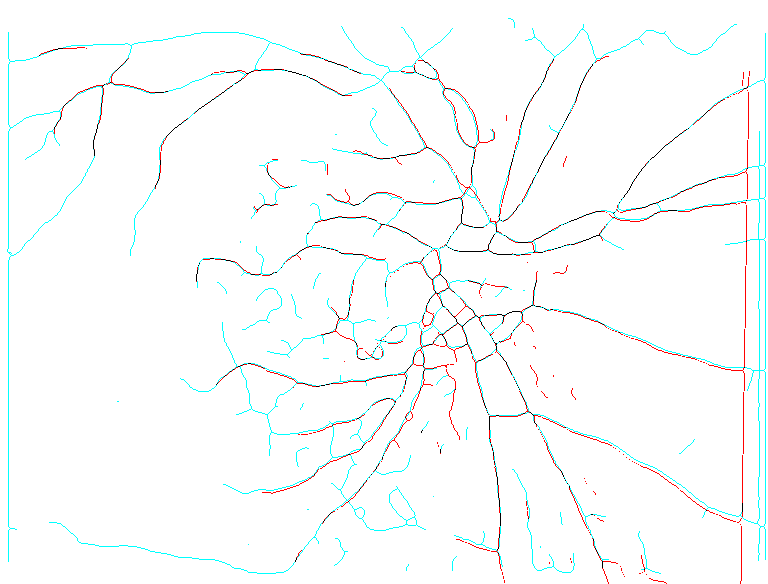
\includegraphics[width=0.9\linewidth]{R122R123-BifurcationGlobal-Skeleton-Registration-0.96393.png}
      \centerline{\footnotesize{(e) BifurcationGlobal方法骨架化配准结果}}\medskip
  \end{minipage}
  \begin{minipage}[b]{0.42\linewidth}
    \centering
    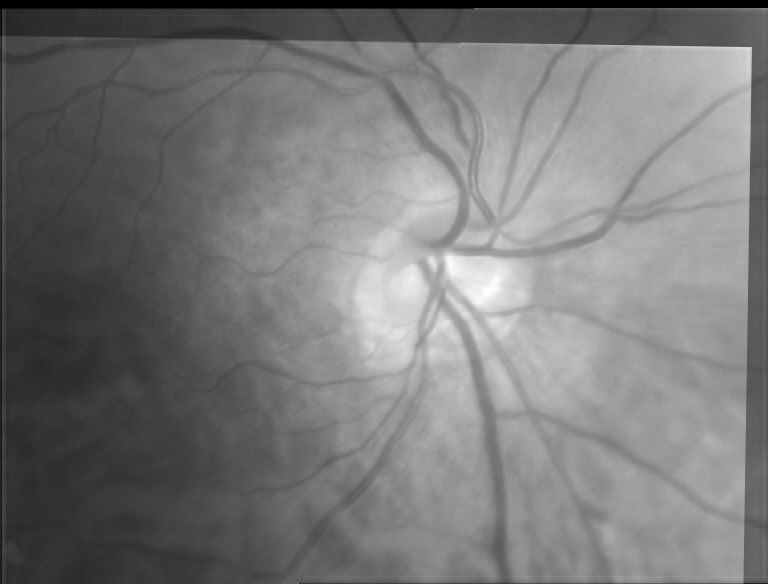
\includegraphics[width=0.9\linewidth]{R122R123-BIfurcationGlobal-Registration.png}
      \centerline{\footnotesize{(f) BifurcationGlobal方法原始图像配准结果}}\medskip
  \end{minipage}
  \\
     \begin{minipage}[b]{0.42\linewidth}
    \centering
    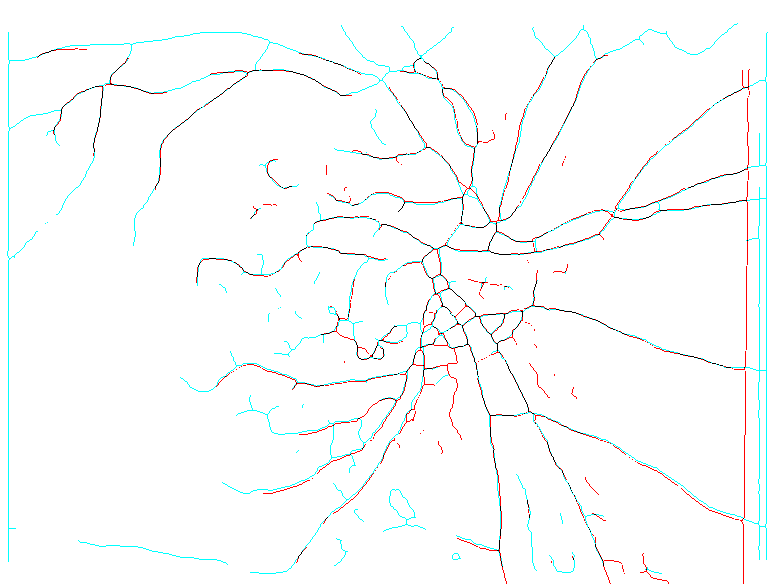
\includegraphics[width=0.9\linewidth]{R122R123-LGMM-Skeleton-Registration-twice-14-five-0.87972.png}
      \centerline{\footnotesize{(g) LGMM方法骨架化配准结果}}\medskip
  \end{minipage}
   \begin{minipage}[b]{0.42\linewidth}
    \centering
    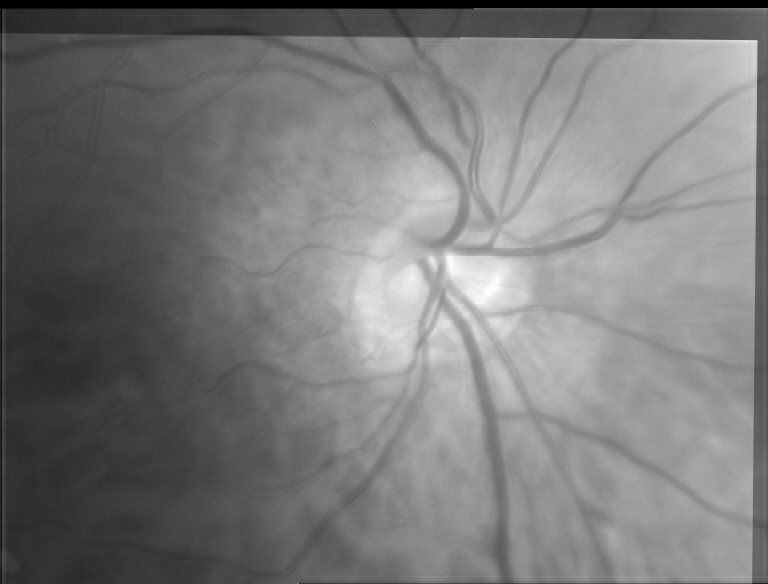
\includegraphics[width=0.9\linewidth]{R122R123-LGMM-Registration.png}
      \centerline{\footnotesize{(h) LGMM方法原始图像配准结果}}\medskip
  \end{minipage}
 \caption{不同方法配准结果一}
\label{m1}
\end{figure}

\begin{figure}
\centering
\begin{minipage}[b]{0.42\linewidth} 
      \centering 
      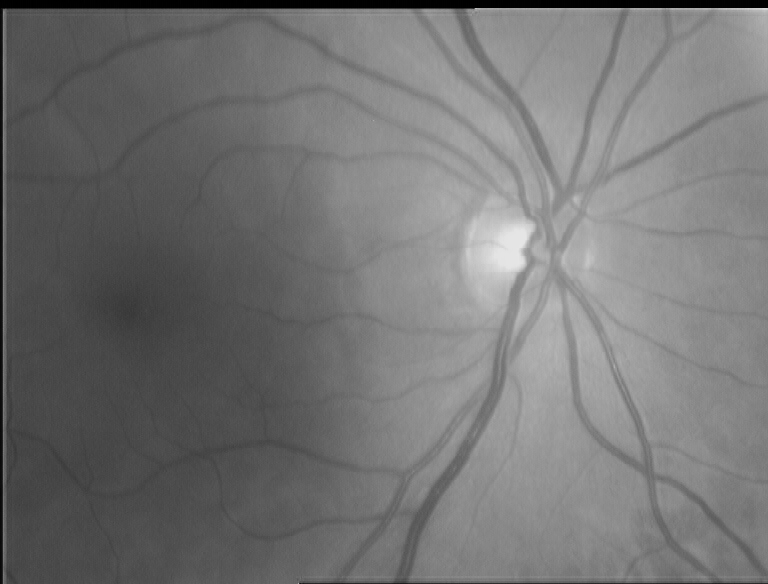
\includegraphics[width=0.9\linewidth]{R210.png}
        \centerline{\footnotesize{(a) 参考图像}}\medskip
\end{minipage}
  \begin{minipage}[b]{0.42\linewidth}
    \centering
    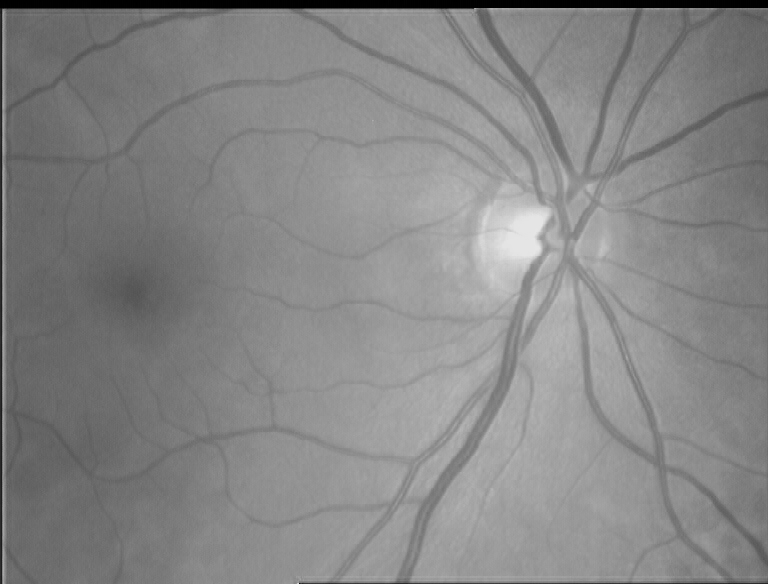
\includegraphics[width=0.9\linewidth]{R209.png}
      \centerline{\footnotesize {(b) 待配准图像}}\medskip
  \end{minipage}
  \\
    \begin{minipage}[b]{0.42\linewidth}
    \centering
    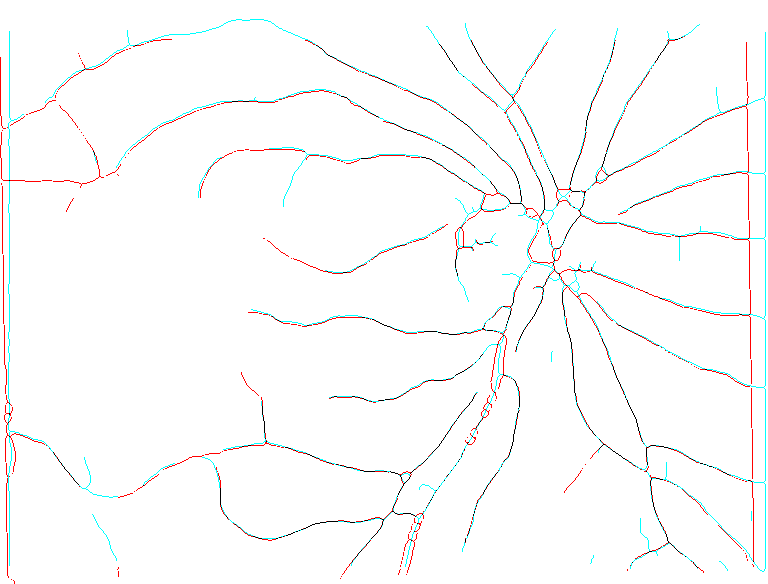
\includegraphics[width=0.9\linewidth]{R210R209-Bifurcation-Skeleton-Registration-1.0223.png}
      \centerline{\footnotesize {(c) Bifurcation方法骨架化配准结果}}\medskip
  \end{minipage}
    \begin{minipage}[b]{0.42\linewidth}
    \centering
    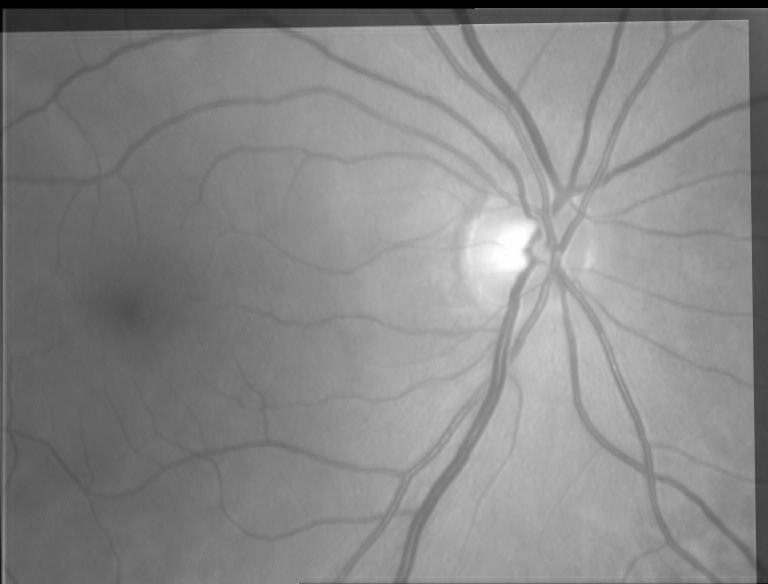
\includegraphics[width=0.9\linewidth]{R210R209-Bifurcation-Registration.png}
      \centerline{\footnotesize {(d) Bifurcation方法原始图像配准结果}}\medskip
  \end{minipage}
  \\
  \begin{minipage}[b]{0.42\linewidth}
    \centering
    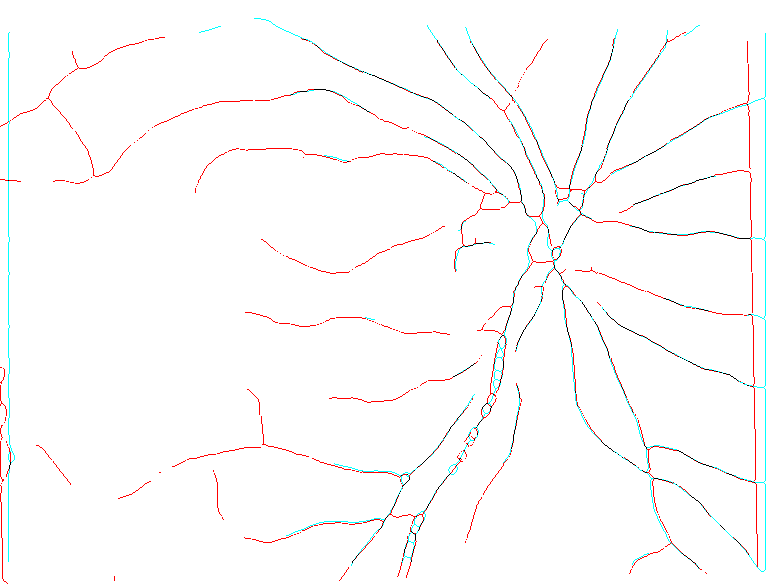
\includegraphics[width=0.9\linewidth]{R210R209-BifurcationGlobal-Skeleton-Registration-0.87467.png}
      \centerline{\footnotesize {(e) BifurcationGlobal方法骨架化配准结果}}\medskip
  \end{minipage}
  \begin{minipage}[b]{0.42\linewidth}
    \centering
    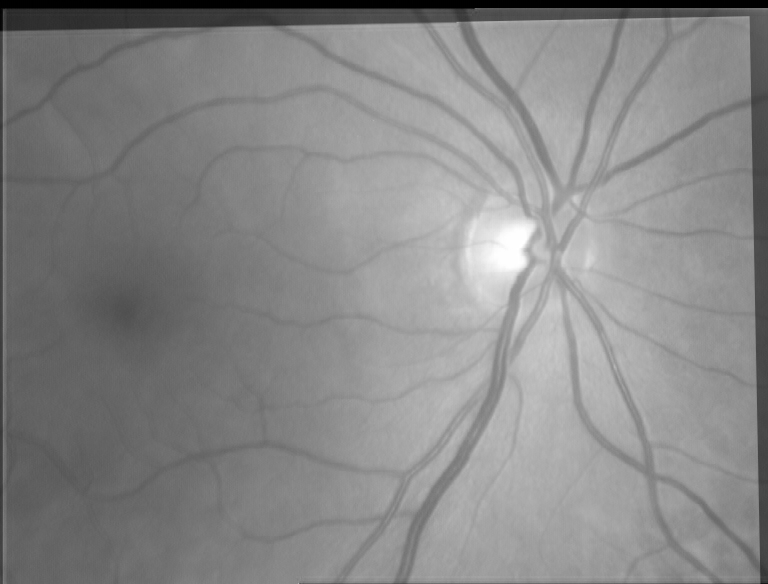
\includegraphics[width=0.9\linewidth]{R210R209-BIfurcationGlobal-Registration.png}
      \centerline{\footnotesize {(f) BifurcationGlobal方法原始图像配准结果}}\medskip
  \end{minipage}
  \\
     \begin{minipage}[b]{0.42\linewidth}
    \centering
    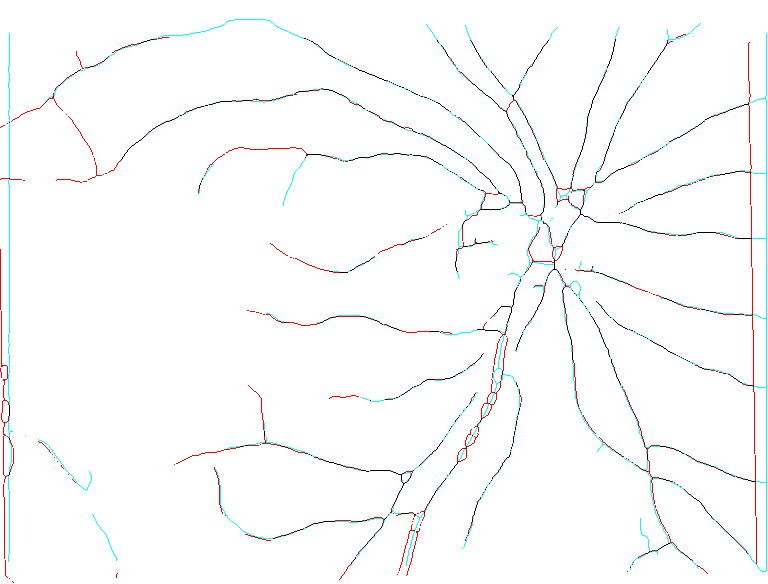
\includegraphics[width=0.9\linewidth]{R210R209-LGMM-Skeleton-Registration-twice-14-three-0.73507.png}
      \centerline{\footnotesize {(g) LGMM方法骨架化配准结果}}\medskip
  \end{minipage}
   \begin{minipage}[b]{0.42\linewidth}
    \centering
    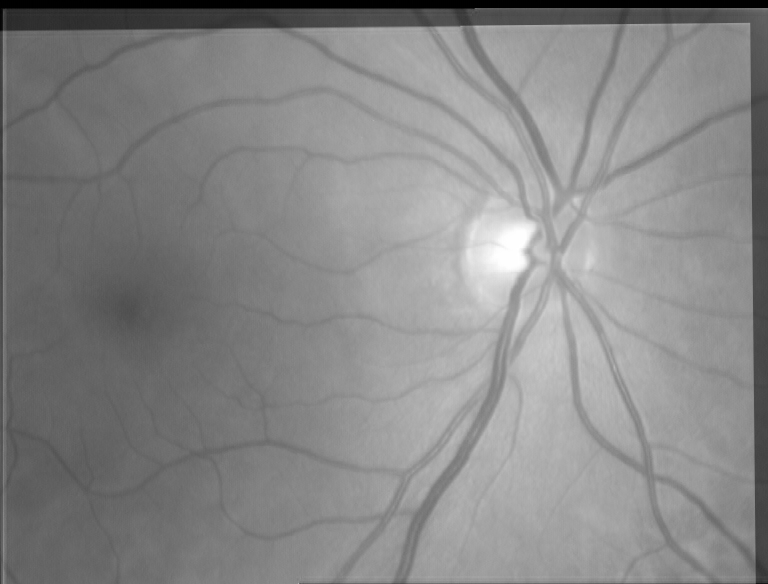
\includegraphics[width=0.9\linewidth]{R210R209-LGMM-Registration.png}
      \centerline{\footnotesize {(h) LGMM方法原始图像配准结果}}\medskip
  \end{minipage}
 \caption{不同方法配准结果二}
\label{m2}
\end{figure} 

\section{本章小结}
本章介绍了一种新的视网膜配准结果度量算法:骨架化对齐误差度量(SAEM)算法,并介绍了本文所做视网膜实验的数据集。着重介绍了多个对比实验:变换模型的对比,配准特征的对比,配准算法的对比。实验结果表明我们的方法在成功率与准确率方面与其他结构方法相比取得了较好的效果:我们提出的环结构与其他特征相比,具有较强的鲁棒性,我们提出的多尺度与从局部到全局的配准策略,对环结构的配准有了巨大的提高,同时在与其他结构特征的结合方面取得了较好的效果,说明了其具有较好的通用性,对于一些结构特征的改进和提高,具有重要意义。
